\section{Design goals}\label{sec:design}

Baltmeri answers a thought experiment: \emph{what if the sea itself had a grammar, and every word in it were decided by a fixed, repeatable procedure applied to the nine languages spoken on its shores?} The design follows from five commitments.

\paragraph{Determinism.} Two people who follow the Manual with the same nine dictionaries must arrive at the same word. No form is chosen by taste; the only human input is the Manual itself. This is what separates Baltmeri from earlier naturalistic auxiliary languages, whose committees exercised judgement at every entry (\S\ref{sec:related-conlang}).

\paragraph{Equity between families.} The nine languages belong to four families with very unequal speaker numbers (Table~\ref{tab:sources}). Voting therefore happens at the \emph{family} level, one family one vote, so that Germanic's three members, or Russian's demographic weight, cannot swamp the others. Inside a family a fixed sub-ranking (Estonian before Finnish, Latvian before Lithuanian, Polish before Russian, Swedish before Danish before German) settles internal disagreement without rotating.

\paragraph{Rotating tie-breaks.} Ties are unavoidable with four voters. They are broken by the \emph{Visby Queue}, a ranking of the nine languages by the distance from Visby on Gotland---the medieval Hanseatic hub in the middle of the sea---to each language's nearest major coastal city. Whichever language breaks a tie moves to the back of the queue (the \emph{Rota Rule}), so that no single language accumulates decisions.

\paragraph{Inheritance before invention.} Where the languages already agree, Baltmeri inherits (the Hanse Rule). Where they disagree, a content word is assigned to the family with the historically richest vocabulary for its semantic domain. Only function words and inflections are put to a plain vote. New morphology is invented nowhere; every ending is the winner of a vote among existing endings.

\paragraph{Pronounceability across the shore.} The sound inventory is restricted to segments at least three of the nine languages produce comfortably, stress is fixed on the first syllable, and a small set of repair rules eliminates clusters that any coastal speaker would stumble over.

These commitments make Baltmeri a \emph{zonal} constructed language in the sense of \S\ref{sec:related-conlang}, but one whose zone is defined by a body of water rather than by a language family, and whose lexicon is generated by an algorithm rather than curated by hand.

\section{Source languages and the Visby Queue}\label{sec:sources}

\begin{table}[t]
\centering\small
\caption{The nine source languages, their families, and the fixed in-family sub-ranking (left to right). Speaker figures are approximate first-language totals and are given only to motivate family-level voting.}
\label{tab:sources}
\setlength{\tabcolsep}{4pt}
\begin{tabular}{@{}lp{3.1cm}ll@{}}
\toprule
Family & Members, ranked & Abbr. & L1 speakers \\
\midrule
Finnic & Estonian, Finnish & et, fi & $\approx$6 M \\
Baltic & Latvian, Lithuanian & lv, lt & $\approx$4.5 M \\
Slavic & Polish, Russian & pl, ru & $\approx$190 M \\
Germanic & Swedish, Danish, German & sv, da, de & $\approx$110 M \\
\bottomrule
\end{tabular}
\end{table}

The Manual fixes the initial queue as
\begin{quote}
Swedish, Latvian, Lithuanian, Estonian, Finnish, Polish, German, Danish, Russian.
\end{quote}
We checked this ordering against great-circle distances from Visby (57.63°N, 18.30°E) to candidate cities (Table~\ref{tab:visby}). The queue is \emph{approximately} geodesic: Stockholm is nearest and Saint Petersburg farthest, as the Manual has it. Two departures are worth recording. Klaipėda (276~km) is nearer than Riga (357~km), so a strict reading would place Lithuanian before Latvian; and if Kaliningrad (353~km) rather than Saint Petersburg (738~km) were taken as Russia's coastal city, Russian would move from last to third. The Manual's queue is therefore best understood as a \emph{convention fixed by the text}, which the engine treats as an axiom, and not as a quantity to be re-measured. Because the queue rotates on every tie, its \emph{state} after the seed lexicon has been derived---the canonical queue, \S\ref{sec:eval-queue}---depends on the order of derivation, which the Manual also fixes (\S3 to \S11, top to bottom).

\begin{table}[t]
\centering\small
\caption{Great-circle distance from Visby to candidate ``nearest major coastal cities'' (haversine, km). Cities in bold are the ones consistent with the Manual's queue.}
\label{tab:visby}
\begin{tabular}{@{}llr@{}}
\toprule
Language & City & km \\
\midrule
Swedish & \textbf{Stockholm} & 189 \\
Lithuanian & \textbf{Klaipėda} & 276 \\
Russian & Kaliningrad & 353 \\
Latvian & \textbf{Riga} & 357 \\
Polish & \textbf{Gdańsk} & 366 \\
Finnish & Turku & 387 \\
Danish & \textbf{Copenhagen} & 412 \\
Estonian & \textbf{Tallinn} & 425 \\
Finnish & \textbf{Helsinki} & 474 \\
German & \textbf{Rostock} & 551 \\
German & Lübeck & 634 \\
Russian & \textbf{Saint Petersburg} & 738 \\
\bottomrule
\end{tabular}
\end{table}

\begin{figure}[t]
\centering
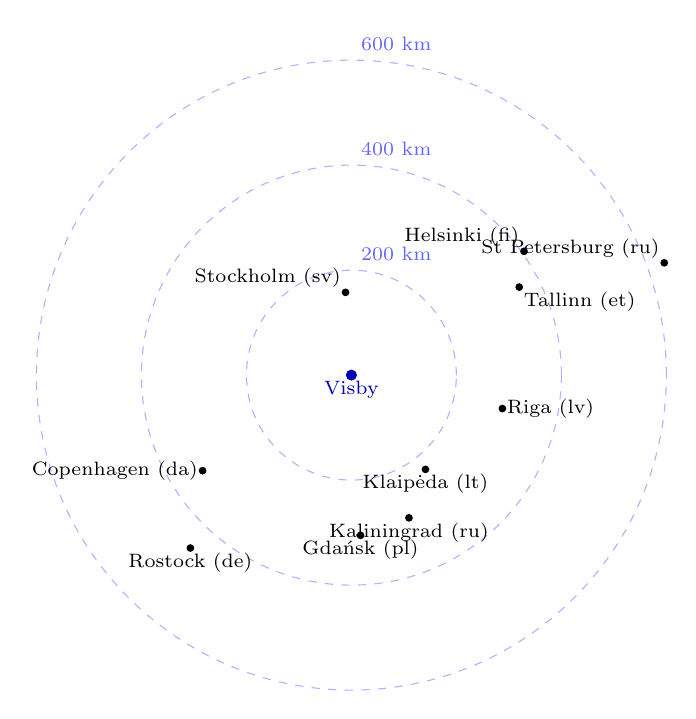
\begin{tikzpicture}[x=0.33cm,y=0.62cm,font=\scriptsize]
  % rings: 200, 400, 600 km  (1 cm = 150 km)
  \foreach \r/\l in {1.333/200 km, 2.667/400 km, 4/600 km} {
    \draw[blue!30,dashed] (0,0) circle [x radius=\r/0.33, y radius=\r/0.62];
    \node[blue!60,anchor=south west] at (0,{\r/0.62}) {\l};
  }
  \fill[blue!70!black] (0,0) circle (2pt) node[anchor=north,inner sep=2pt] {Visby};
  \foreach \lon/\lat/\name/\pos in {
    18.069/59.329/Stockholm (sv)/above left,
    24.105/56.949/Riga (lv)/right,
    21.144/55.703/Klaipėda (lt)/below,
    24.754/59.437/Tallinn (et)/below right,
    24.938/60.170/Helsinki (fi)/above left,
    18.646/54.352/Gdańsk (pl)/below,
    12.099/54.092/Rostock (de)/below,
    12.568/55.676/Copenhagen (da)/left,
    30.335/59.934/St~Petersburg (ru)/above left,
    20.510/54.710/Kaliningrad (ru)/below} {
    \fill[black] ({\lon-18.295},{\lat-57.634}) circle (1.4pt) node[\pos,inner sep=1.5pt] {\name};
  }
\end{tikzpicture}
\caption{The Visby Queue as geography: equirectangular sketch of the nine languages' coastal cities around Visby, with 200, 400 and 600 km rings. Kaliningrad, the Russian city the Manual does not use, is the Russian city the Manual does not use; it would place Russian third.}
\label{fig:visby}
\end{figure}
